\documentclass[12pt, a4paper]{article}
%
%%%%%%%%%%%%%%%%%%%%%%%%%%%%%%%%%%%%%%%%%%%%%
% SWITCH FOR PDFLATEX or LATEX
%%%%%%%%%%%%%%%%%%%%%%%%%%%%%%%%%%%%%%%%%%%%%
%%%
\ifx\pdfoutput\undefined %% LATEX %%%%%%%%%%%
%%%
\usepackage[dvips]{graphicx}
\DeclareGraphicsExtensions{.eps}
\usepackage[ps2pdf]{thumbpdf}
\usepackage[ps2pdf,
bookmarks=true,bookmarksnumbered=true,%
hypertexnames=false,%
breaklinks=true,%
linkbordercolor={0 0 1},pdfborder={0 0 112.0}]{hyperref}
%
\hypersetup{
pdfauthor   = {Patrick J\"{o}ckel <patrick.joeckel@dlr.de>},
pdftitle    = {NCREGRID MANUAL},
pdfsubject  = {},
pdfkeywords = {},
pdfcreator  = {LaTeX with hyperref package},
pdfproducer = {dvips + ps2pdf}
}
%%%
\else %% PDFLATEX %%%%%%%%%%%%%%%%%%%%%%%%%%%%%%%
%%%
\usepackage[pdftex]{graphicx} % pdfLaTeX
\DeclareGraphicsExtensions{.pdf}
\usepackage[pdftex]{thumbpdf}
\usepackage[pdftex,
bookmarks=true,bookmarksnumbered=true,%
hypertexnames=false,%
breaklinks=true,%
linkbordercolor={0 0 1}]{hyperref}
\hypersetup{
pdfauthor   = {Patrick J\"{o}ckel <patrick.joeckel@dlr.de>},
pdftitle    = {NCREGRID MANUAL},
pdfsubject  = {},
pdfkeywords = {},
}
\pdfadjustspacing=1 %% ENSURE LATEX-like spacing
%%%
\fi  %% END OF PDFLATEX
%%%
%%%%%%%%%%%%%%%%%%%%%%%%%%%%%%%%%%%%%%%%%%%%%%%%%%%%%%%
%
\setcounter{secnumdepth}{4}
\setcounter{tocdepth}{4}
%
%%%%%%%%%%%%%%%%%%%%%%%%%%%%%%%%%%%%%%%%%%%%%%%%%%%%%%%
\title{NCREGRID - Version 1.4b\\ Documentation}
\author{Patrick J\"{o}ckel
  \footnote{Deutsches Zentrum f\"ur Luft- und Raumfahrt (DLR),
    Institut f\"ur Physik der Atmosph\"are, Oberpfaffenhofen,
    82234 We{\ss}ling, Germany}
(patrick.joeckel@dlr.de)}
\date{\today}
%
\begin{document}
%
\maketitle
%
\begin{abstract}
NCREGRID is a tool for data transformation of gridded 2- and
3-di\-men\-sio\-nal (spatial) geophysical/geochemical scalar fields
between grids of different resolutions.
The program handles data on rectangular latitude/longitude grids
(not necessarily evenly spaced and/or monotone)
and vertical pressure hybrid grids of arbitrary resolution.
The input/output data format is {\it netCDF}.
The NCREGRID core is a recursive algorithm (NREGRID) which is applicable
to arbitrary (curvilinear) grids (with orthogonal axes) of any dimension
and not restricted to geo\-phy\-si\-cal / geo\-chemi\-cal global hybrid grids.
NCREGRID is freely available without any warranty under the GNU public license.
\end{abstract}

\section*{Reference}
J\"ockel, P.: Technical note: Recursive rediscretisation of geo-scientific data
in the Modular Earth Submodel System (MESSy), Atmospheric Chemistry and
Physics, 6, 3557–3562, doi: 10.5194/acp-6-3557-2006, URL:
\url{https://doi.org/10.5194/acp-6-3557-2006} (2006).

\clearpage
\tableofcontents
\clearpage

%%%%%%%%%%%%%%%%%%%%%%%%%%%%%%%%%%%%%%%%%%%%%%%%%%%%%%%%%%%%%%%%%%%%%%%%%%%%%

\section{Introduction}
\label{sec:intro}
%%%%%%%%%%%%%%%%%%%%%%
In 3-dimensional global geophysical/geochemical modelling 
solving of sets of differential equations describing a
geophysical/geochemical system in the space time domain is often performed
by discretisation with the Eulerian approach, i.e., on a discrete
grid of spatial coordinates.
For this, model input parameters need to be available on 2- or
3-dimensional (2D, 3D) grids of various resolutions.
The horizontal grid space usually comprises geographical latitude and
longitude. Especially in 3D global atmospheric models 
the vertical pressure ($p$) coordinate
is often defined as a set of hybrid levels (with index $i$) of the form
\begin{equation}
 \label{e:hybrid}
    p(i,x,y,t) = h_a(i) \cdot p_0 + h_b(i) \cdot p_s(x,y,t)~~,
\end{equation}
where $p_s$ is the surface pressure, $p_0$ is a constant reference pressure,
and $h_a$ and $h_b$ are the hybrid coefficients. This representation in a
curvilinear coordinate system
(dependent on longitude $x$, latitude $y$, and time $t$)
allows a terrain following vertical coordinate, if $h_a = 0$ and
$h_b = 1$ for the lowest level (surface level).

A wide variety of grid resolutions is used in different models
and for different purposes. Moreover, global geophysical/geochemical data
(also observations) are provided in different spatial resolutions.
As a consequence, data sets have often to be adapted to a specific
grid resolution.
For this purpose, NCREGRID was implemented.

NCREGRID can be used as a stand-alone program, and/or coupled as an import
interface to a model, in order to regrid automatically the input from an
arbitrary grid space onto the required grid resolution. 

The regridding is performed by a recursive algorithm, which itself is
applicable to arbitrary rectangular (curvilinear) grids (with orthogonal axes)
of any dimension,
and not restricted to geo-hybrid-grid structures as described above.

%%%%%%%%%%%%%%%%%%%%%%%%%%%%%%%%%%%%%%%%%%%%%%%%%%%%%%%%%%%%%%%%%%%%%%%%%%%%%

\section{License}
\label{sec:license}
%%%%%%%%%%%%%%%%%%%
The NCREGRID software is free software; it can be redistributed and/or
modified under the terms of the GNU General Public License
as published by the Free Software Foundation; either version 2
of the License, or any later version,
and under additional agreements for scientific software
as described in the file {\it LICENSE.txt} delivered with this distribution.

This program is distributed in the hope that it will be useful,
but WITHOUT ANY WARRANTY; without even the implied warranty of
MER\-CHAN\-TA\-BI\-LI\-TY or FITNESS FOR A PARTICULAR PURPOSE.  See the
GNU General Public License for more details.

A copy of the GNU General Public License ({\it GPL.txt}) should have
been shipped
along with this distribution; if not, it can be received from the Free Software
Foundation, Inc., 59 Temple Place - Suite 330, Boston, MA  02111-1307, USA.

%%%%%%%%%%%%%%%%%%%%%%%%%%%%%%%%%%%%%%%%%%%%%%%%%%%%%%%%%%%%%%%%%%%%%%%%%%%%%

\section{Prerequisites}
\label{sec:prerequisites}
%%%%%%%%%%%%%%%%%%%%%%%%%
NCREGRID is written in Fortran95, thus a Fortran95 compiler
is required for installation of the software.
(A Fortran90 compiler which is capable to handle initialisation
statements in declaration lines should do as well.)
%
Furthermore, {\it (g)make} is used for building the software.

Since the input and output format is {\it netCDF}\\
(http://www.unidata.ucar.edu/packages/netcdf/),\\
the Fortran90 version (i.e., at least {\it netCDF} - Version 3.6.0)
of the {\it netCDF} library is required.
%% Due to a known problem of {\it netCDF} version 3.5.0\\
%% (see http://www.unidata.ucar.edu/packages/netcdf/known\_problems.html\#j90)
%% an update to {\it netCDF} version 3.5.1b might be necessary.
%% Note that in this distribution the file {\it src/f90/netcdf\_variables.f90}
%% contains a line that might cause problems on some compilers.
%% Please change
%% \begin{verbatim}
%%     if(present(dimids)) dimids(:numDimensions) = dimensionIDs(:)
%% \end{verbatim}
%% to
%% \begin{verbatim}
%%     if(present(dimids)) dimids(:numDimensions) =    &
%%                         dimensionIDs(:numDimensions)
%% \end{verbatim}

NCREGRID comprises the {\it f2kcli} command line interface\\
(http://www.winteracter.com/f2kcli/index.htm)\\
for the stand-alone version.

%%%%%%%%%%%%%%%%%%%%%%%%%%%%%%%%%%%%%%%%%%%%%%%%%%%%%%%%%%%%%%%%%%%%%%%%%%%%%

\section{Installation}
\label{sec:installation}
%%%%%%%%%%%%%%%%%%%%%%%%
The installation is straightforward:
\begin{enumerate}
\item unpack the archive:\\
      {\bf uncompress ncregrid.tar.Z}\\
      {\bf tar xvf ncregrid.tar}\\
\item change to the subdirectory {\it ./ncregrid}:\\
      {\bf cd ncregrid}
\item configure NCREGRID according to your system:\\
      {\bf ./configure VARIABLE=VALUE ...}\\
      with possible VARIABLEs:\\
      \begin{tabular}{lll}
        {\bf F90}      & name of the Fortran90/95 compiler    & (optional)\\
        {\bf F90FLAGS} & Fortran90/95 compiler options        & (required)\\
                       & (e.g., option for invoking the cpp preprocessor) & \\
        {\bf NC\_INC}  & (absolute) path where {\it netcdf.mod} &\\
                       & is located                          & (required)\\
        {\bf NC\_LIB}  & (absolute) path where {\it libnetcdf.a} &\\
                       & is located                          & (required)\\
      \end{tabular}
      Platform/Compiler specific notes can be found in the {\it README} file
      of the distribution.
\item build the executable and the modules:\\
      {\bf gmake}
\item move the executable and the modules to the {\it ./bin} and
      {\it ./include}
      subdirectories, respectively:\\
      {\bf gmake install}
\item clean-up the source directory:\\
      {\bf gmake clean}
\end{enumerate}
%
The executable {\bf ncregrid.exe} should now be available in the
{\it ./bin} subdirectory, the modules in the {\it ./include}
subdirectory of ncregrid.
The status after unpacking the archive can be achieved
with {\bf gmake distclean}.

%%%%%%%%%%%%%%%%%%%%%%%%%%%%%%%%%%%%%%%%%%%%%%%%%%%%%%%%%%%%%%%%%%%%%%%%%%%%%

\section{Tested Systems}
\label{sec:systems}
%%%%%%%%%%%%%%%%%%%%%%%%
NCREGRID has been tested so far on/with the following platforms/compilers:
\begin{itemize}
\item PC (i686) Linux-2.4.18 (SuSE 8.0) with\\
      lf95 (Lahey/Fujitsu Fortran 95 Express Release L6.10a)
\item Dec-Alpha OSF1-4.0f with\\
      f90 (Compaq Fortran 90 (formerly DIGITAL Fortran 90))
\item Dec-Alpha OSF1-5.1a with\\
      f90 (Compaq Fortran 90 (formerly DIGITAL Fortran 90))
\item Silicon Graphics Origin 2100
\item Windows 98 with Compaq Visual Fortran
\item IBM-AIX
\item SGI Origin 3800, IRIX6.5 with MIPSpro 7
\item NEC-SX6
\item PC (i686) Linux-2.4.20 (SuSE 8.2) with\\
      NAG-f90
\end{itemize}
If you succeed to build NCREGRID on platforms which are not listed here,
please send an e-mail with system/compiler information, potential
changes/extensions to the source code, and/or the Makefile to
{\it patrick.joeckel@dlr.de}.

%%%%%%%%%%%%%%%%%%%%%%%%%%%%%%%%%%%%%%%%%%%%%%%%%%%%%%%%%%%%%%%%%%%%%%%%%%%%%

\section{Usage}
\label{sec:usage}
%%%%%%%%%%%%%%%%%
NCREGRID can be applied in two different modes:
\begin{itemize}
 \item Stand-allone mode for the rediscretization of data files in
       {\it netCDF}
 \item Interface mode (coupled to a model)
       for automatic rediscretisation during data import from {\it netCDF}
       files
\end{itemize}
%
In both models, the application of NCREGRID is basically performed
in 4 steps:
%
\begin{enumerate}
\item Analysis of the {\it netCDF} file containing the data which should be
      regridded ($<$infile$>$). This can for instance be done with:\\
      {\bf ncdump -h $<$infile$>$}\\       
      Required are the names of the {\it netCDF} variables spanning the
      grid (such as latitude, longitude, surface pressure, reference pressure,
      hybrid-co\-efficients, time), and the names of the variables which
      should be regridded.
      Note that this step is left to the user, in order to be independent
      of specific {\it netCDF} conventions.
      Note further that {\it netCDF} and NCREGRID are case-sensitive.
\item Analysis of the output grid structure:\\
      \begin{itemize}
      \item The output grid structure is available in a {\it netCDF} file:\\
            The information from that file ($<$grdfile$>$) can be extracted
            from this file in analogy to step 1. above.
      \item NCREGRID is used in interface mode:\\
            The output grid information is provided
            by the grid-specification
            interface (see section~\ref{sec:defineinterface})
      \item The output grid structure is not available:\\
            The output grid information can be written with an appropriate
            text editor in the CDL-syntax (see {\it netCDF}-manual).
            From this, a {\it netCDF} file can be generated by\\
            {\bf ncgen -b -o $<$grdfile$>$ $<$cdl-file$>$}\\
            and used as $<$grdfile$>$, as above.
      \end{itemize}
\item Summary of all required information in a namelist:\\
      The NCREGRID namelist structure is described in detail in
      section~\ref{sec:namelist}.
\item Start NCREGRID:\\
      \begin{itemize}
      \item NCREGRID in stand-alone mode:\\
            {\bf ncregrid $<$namelist-file$>$}
      \item NCREGRID in interface mode:\\
            start the executable with NCREGRID linked\\
            Detailed information about the usage of NCREGRID from
            Fortran90/Fortran95 code is provided in
            section~\ref{sec:startinterface}.
      \end{itemize}
\end{enumerate}

%%%%%%%%%%%%%%%%%%%%%%%%%%%%%%%%%%%%%%%%%%%%%%%%%%%%%%%%%%%%%%%%%%%%%%%%%%%%%

\section{Namelist Control}
\label{sec:namelist}
%%%%%%%%%%%%%%%%%%%%%%%%%%%%%%%%%%%
The regridding procedure of NCREGRID is controlled by a
namelist (and some optional control parameters
specified at the subroutine call of {\bf REGRID\_CONTROL}, if NCREGRID is
used in interface mode).
The syntax of a NCREGRID namelist is:
\begin{verbatim}
    &regrid
    variable = value,
    ...
    /
\end{verbatim}
The dots indicate a list of further namelist entries.
Several namelists can be concatenated into one $<$namelist-file$>$.
These namelists are
then processed by NCREGRID in sequence.
Table~\ref{tab:namelist} gives an overview of the possible namelist entries
with their meanings.
%
\begin{table}
 \centering
\begin{tabular}{|l|l||l|}
\hline
  INPUT &OUTPUT & Description\\
\hline
\hline
  infile      & outfile     & input/output {\it netCDF} file\\
  grdfile     &             & {\it netCDF} file with output grid\\
  i\_lat(m/i) & g\_lat(m/i) & name of latitude axis\\
  i\_latr     & g\_latr     & range of latitude axis\\
  i\_lon(m/i) & g\_lon(m/i) & name of longitude axis\\
  i\_lonr     & g\_lonr     & range of longitude axis\\
  i\_hya(m/i) & g\_hya(m/i) & name of hybrid-A-coeff.\\
  i\_hyar     & g\_hyar     & range of hybrid-A-coeff.\\
  i\_hyb(m/i) & g\_hyb(m/i) & name of hybrid-B-coeff.\\
  i\_hybr     & g\_hybr     & range of hybrid-B-coeff.\\
  i\_time(m/i)& g\_time(m/i)& name of time axis\\
  i\_ps       & g\_ps       & name/value of surface pressure\\
  i\_p0       & g\_p0       & name/value of reference pressure\\
  i\_t        & o\_t        & input/output time step control\\
  g\_t        &             & grid time step control\\
\hline
  var         &             & variable list\\
  pressure    &             & vert. regridding in pressure coord.\\
  input\_time &             & output file gets input time axis\\
\hline
\end{tabular}
\caption[List of NCREGRID namelist variables]
{List of NCREGRID namelist variables. With (...m/...i) the
box mid point coordinates (...m) and/or the box interfaces (...i),
are specified, respectively.
i\_t(4), o\_t(3), and g\_t(3) are integer vectors, pressure 
and input\_time are of type logical,
i/g\_latr, i/g\_lonr, i/g\_hyar, and i/g\_hybr are real vectors
of length 2, 
all others are character/string variables.}
\label{tab:namelist}
\end{table}

\subsection{Grid specification}
\label{sec:grid}
In order to allow {\it netCDF}-files to be as general as possible,
and not to be restricted to specific {\it netCDF}-conventions,
the input grid (read from the {\it netCDF} file $<$infile$>$) has to be
specified by the user via the namelist.
With the namelist variables {\bf i\_lat(i/m)}, {\bf i\_lon(i/m)},
{\bf i\_hya(i/m)}, {\bf i\_hyb(i/m)}, {\bf i\_ps}, and {\bf i\_p0}
a 3D input grid (spatial) is fully described.
The output grid ({\bf g\_...}) is specified in analogy, and read from the
$<$grdfile$>$. The output is written to the {\it netCDF} file
$<$outfile$>$.
%

For the regridding procedure,
the interfaces ({\bf i...}) of the grid boxes are required (except for
{\bf i/g\_timei}).
If the respective data is not available in the $<$infile$>$/$<$grdfile$>$,
or the entries are not present in the namelist, the interface values are
internally calculated from the corresponding mid-box values,
assuming that the interfaces are half-way between the mid-points.
The outer interfaces are calculated using the same distance
between outermost mid-point and corresponding inner interface.
If this calculation of the outer interfaces is not applicable, the user
can specify them with the namelist variables {\bf i\_latr}, {\bf i\_lonr},
{\bf i\_hyar}, {\bf i\_hybr} for the input grid, and with
{\bf g\_latr}, {\bf g\_lonr}, {\bf g\_hyar}, {\bf g\_hybr} for the output grid,
respectively.
For example,
\begin{verbatim}
    ...
    i_latm = 'latitude',
    i_latr = -90.0, 90.0,
    ...
\end{verbatim}
in the namelist ensures that the outer input grid
latitude interfaces (calculated from the mid-box latitudes with name
'latitude') are at -90.0$^o$ and 90.0$^o$.
Note that in case of {\bf i/g\_hyar} the order of parameters is relevant,
since the hybrid-A-coefficients (see Eq.~(\ref{e:hybrid})) are not
monotone. Therefore, in
\begin{verbatim}
    i_hyar = a1, a2,
\end{verbatim}
'a1' refers to the highest grid level (corresponding to the smallest
hybrid-B-coefficient (!)), and 'a2' to the lowest grid level (corresponding to
the largest hybrid-B-coefficient (!)), respectively.

Since the core of NCREGRID (NREGRID, see section~\ref{sec:nregrid})
performs regridding in rectangular grid space without weighting,
the latitude axis intervals have to be weighted according to the surface.
Therefore, NCREGRID uses internally 
\begin{equation}
  \label{e:latitude}
  cos(((latitude(:) - 90)/180) \cdot \pi)
\end{equation}
for regridding along the latitude axes (see {\it messy\_ncregrid\_geohyb.f90},
{\bf SUBROUTINE GEOHYBGRID\_AXES}).

If the interface variables are specified in the namelist, but not the
corresponding mid-points, the latter are internally calculated,
assuming that the mid-points are half-way between the interfaces.
The mid-points, however, are not used by the regridding procedure.

Dimensions defined for the input grid ($<$infile$>$),
but omitted for the output grid ($<$grdfile$>$) are treated as invariant
(see section~\ref{sec:opseq}).

\subsection{Syntax of the namelist variable var}
\label{sec:varstr}
With the namelist variable {\bf var} the user specifies the scalar
fields of the
$<$infile$>$ (which have to be on the specified input-grid) that should be
regridded. For output to the $<$outfile$>$, the variables can be renamed and
scaled. Moreover, the regridding type (see section~\ref{sec:rgtypes})
can be assigned. The syntax is
\begin{verbatim}
    var = '[new_name=]name[:RG_TYPE][,scale]; ...',
\end{verbatim}
whereby the dots indicate a list of further variables.
'name' is the variable name
in $<$infile$>$, 'new\_name' is the variable name in $<$outfile$>$,
'RG\_TYPE' is the regridding type (see section~\ref{sec:rgtypes}),
and 'scale' is the scaling factor. The
order of ':RG\_TYPE' and ',scale'  is arbitrary.

If 'new\_name' is omitted, the variable is not renamed. If 'scale'
is omitted, the variable is not scaled.
If 'RG\_TYPE' is omitted, NCREGRID checks the $<$infile$>$
for the variable attribute 'RG\_TYPE'. If this attribute is not set,
or the value is not recognised, NCREGRID takes 'INT' as default
(see section~\ref{sec:rgtypes}).

If the namelist variable {\bf var} is not specified at all, NCREGRID scans the
$<$infile$>$ for all variables on the specified input grid. Renaming and
scaling are not performed. The regridding type
is set to 'INT', unless the variable attribute 'RG\_TYPE' in
$<$infile$>$ is specified.

\subsection{Time control}
\label{sec:tctrl}
With the time control namelist variables {\bf i\_t}, {\bf g\_t} and {\bf o\_t}
the user specifies the time-steps of {\it netCDF}-variables for regridding.
The syntax is
\begin{verbatim}
    i_t = itmin,itstep,itmax,itret,  ! default: 1, 1, 0, 0
    g_t = gtmin,gtstep,gtreset,      ! default: 1, 1, 0
    o_t = otstart,otstep,otdummy     ! default: 1, 1, 0
\end{verbatim}
where {\bf itmin}, {\bf itstep}, {\bf itmax}, {\bf itret},
{\bf gtmin}, {\bf gtstep}, {\bf gtreset},
{\bf otstart}, and {\bf otstep} are integers
The default settings are listed above.
The third entry of {\bf o\_t} ({\bf otdummy}) is currently not used.

NCREGRID resets automatically {\bf itstep}, {\bf gtstep}, and/or {\bf otstep}
to 1, if 0 is specified in the namelist; {\bf itmax} and {\bf itret} are set to
{\bf itmin}, if not specified in the namelist.
The overall consistency of all time step control parameters is checked
by NCREGRID, and documented by the output of error/warning messages,
if required.

The input variables are regridded between {\bf itmin} and {\bf itmax} with a
step size of {\bf itstep}. The regridded data of time step {\bf itret} are
returned to the {\bf REGRID\_CONTROL} subroutine call
(i.e., {\bf itret} has no meaning in the stand-alone mode of NCREGRID).

For the destination grid of the variables at the input time steps
({\bf itmin}, {\bf itmin+itstep}, {\bf itmin+2*itstep}, {\bf ...}, {\bf itmax})
the grid from $<$grdfile$>$
is used at time step {\bf gtmin}, {\bf gtmin+gtstep},
{\bf gtmin+2*gtstep}, {\bf ...} , respectively.
If {\bf gtreset} is reached, the $<$grdfile$>$ time step
is reset to {\bf gtstart} again, etc.
(This allows for instance the regridding of 60 time steps of monthly averaged
data (in $<$infile$>$), to a grid (in $<$grdfile$>$) which is only known
climatologically, i.e. containing 12 monthly averages.

And finally, the regridded data is written to the output file with
time steps {\bf otstart}, {\bf otstart+otstep}, {\bf otstart+2*otstep},
{\bf ...} .
This is needed, e.g., if {\bf itstep} is not 1, but the $<$outfile$>$
should contain a continuous time series.

With the namelist variable {\bf input\_time} the time axis specification in the
output file ($<$outfile$>$) is set. Per default ({\bf input\_time = T}) 
the $<$outfile$>$ time axis is the same as in $<$infile$>$.
Otherwise, ({\bf input\_time = F}) the $<$grdfile$>$ time axis
(or interface time axis in interface mode) is taken for $<$outfile$>$.
%
Additionally, in interface mode the output time stepping
({\bf o\_t}) is set to the $<$infile$>$ time stepping (in case of
{\bf input\_time=T}), or to the interface time
stepping (in case of {\bf input\_time = F}), respectively.

\subsection{Vertical axis specifications}
NCREGRID is capable to handle all cases of vertical
pressure axes, such as
\begin{itemize}
\item hybrid pressure axes ($h_a \neq 0$, $h_b \neq 0$);
\item constant pressure axes ($h_b = 0$); {\bf i/g\_hybi/m} omitted in namelist
\item sigma levels ($h_a = 0$);  {\bf i/g\_hyai/m} omitted in namelist
\end{itemize}

\subsubsection{Surface and reference pressure}
If the surface pressure and/or reference pressure is/are not contained
in $<$infile$>$ and/or $<$grdfile$>$, respectively, or they should not
be used, it is possible to specify a constant value, for example:
\begin{verbatim}
    i_p0 = '101300.0 Pa'
\end{verbatim}
The syntax is the same for {\bf g\_p0}, {\bf i\_ps}, and {\bf g\_ps}.
Note that in these cases the unit must be chosen such that surface pressure,
reference pressure and the hybrid-coefficients are consistent
(see Eq.~(\ref{e:hybrid})).
The unit ('Pa' in the specification above) is only converted to
the {\it netCDF} variable attribute 'units' in the output file,
but, not used internally for automatic unit conversions!

\subsubsection{Vertical regridding coordinates}
Calculation of the vertical overlap of grid-boxes between $<$infile$>$ and
$<$grdfile$>$ is internally performed in sigma-coordinates per default
\begin{equation}
 \sigma(i) = p(i,x,y,t)/p_s(x,y,t)~,
\end{equation}
in order to avoid conservation problems in case the source and destination
surface pressure fields are different.
However, a vertical regridding in pressure coordinates can be
enforced, if the variable {\bf pressure = T} is specified in the namelist.
Note, however, that in such cases input and output
pressure levels must have the same units!

\subsection{Namelist examples}
Examples of NCREGRID namelists can be found in the\\
{\it ./ncregrid/examples/namelist}
subdirectory of this distribution.

%%%%%%%%%%%%%%%%%%%%%%%%%%%%%%%%%%%%%%%%%%%%%%%%%%%%%%%%%%%%%%%%%%%%%%%%%%%%%

\section{Regridding Types}
\label{sec:rgtypes}
%%%%%%%%%%%%%%%%%%%%%%%%%%
The core of NCREGRID, NREGRID (see section~\ref{sec:nregrid}),
is designed to rediscretize arbitrary distributions from
one grid to another, without adding information (e.g., if regridding from
a coarser to a finer grid), or reducing more information
than is lost anyway (e.g., if regridding from a finer to a coarser
grid). {\bf Thus, no inter-/extrapolation methods are applied!}
The data fields are purely redistributed, assuming constant values
within one grid box,
represented by the grid box mid point. For this, intensive and
extensive variables are distinguished.

Accordingly, the following regridding types (RG\_TYPE) are supported
at present
for the regridding of variables (scalar fields!) between geo-hybrid grids:
%
\begin{itemize}
\item INT: INT is suitable for intensive quantities, such as
           tracer mass mixing ratios, or temperature fields. This option
           conserves the global weighted average
           of a scalar field during the regridding procedure.
\item EXT: EXT is suitable for extensive quantities, such as
           tracer masses, or tracer emission maps (2D). This option 
           conserves the global unweighted sum over all grid boxes of a 
           scalar field.
\item IDX: IDX is suitable for regridding index distributions, i.e.,
           scalar fields with discrete values, where averaging is not
           defined. The index-regridding returns for a given
           destination grid-box the index, which has in all
           overlapping source grid-boxes the largest relative contribution.
\item IXF: IFX is similar to IDX, however it returns a variable extended by
           one dimension, whereby the additional dimension is along the
           index range.
           A given slice along the new index-dimension contains the
           fraction of that index in the respective grid-box.
\end{itemize}

%%%%%%%%%%%%%%%%%%%%%%%%%%%%%%%%%%%%%%%%%%%%%%%%%%%%%%%%%%%%%%%%%%%%%%%%%%%%%

\section{NCREGRID in Interface Mode}
\label{sec:interface}
%%%%%%%%%%%%%%%%%%%%%%%%%%%%%%%%%%%%%%%%%%%%%%%%%
The usage of NCREGRID in interface mode, i.e., linked to another program,
requires two steps:
\begin{itemize}
  \item specification of the destination grid in the Fortran95 code
  \item calling the regridding procedure from the Fortran95 code
\end{itemize}

\subsection{Destination grid definition}
\label{sec:defineinterface}
For NCREGRID in interface mode (e.g., as part of a model)
a specification of the destination grid in the Fortran95 code is required,
which provides the informations about the destination grid,
as alternative to the specification via the {\bf grdfile} entry in the
namelist (see section~\ref{sec:namelist}). 
%
This definition section is contained
in the module {\it messy\_ncregrid\_interface.f90}
An example can be found in the
{\it ./ncregrid/examples/interface} subdirectory.
%
The grid definition module provides two subroutines:
\begin{itemize}
\item {\bf SUBROUTINE INTERFACE\_GEOHYBGRID}:
      returns the grid information as a Fortran95 structure
      ({\bf TYPE geohybgrid}, \\
      see {\it messy\_ncregrid\_geohyb.f90},
      see section~\ref{sec:struct})
\item {\bf SUBROUTINE INTERFACE\_SET\_MESSAGEMODE}:
      controls the degree of diagnostic output of NCREGRID;
      The following parameters can be used, i.e. summed
      (MSGMODE = ... + ... + ):
        \begin{tabular}{ll}
          {\bf MSGMODE\_S}  & silent\\
          {\bf MSGMODE\_E}  & error messages\\
          {\bf MSGMODE\_VL} & little verbose\\
          {\bf MSGMODE\_W}  & warning messages\\
          {\bf MSGMODE\_VM} & medium verbose\\
          {\bf MSGMODE\_I}  & info messages\\
        \end{tabular}
\end{itemize}

\subsection{Calling NCREGRID from Fortran95 code}
\label{sec:startinterface}
%
\subsubsection{Level 1 (low level) user interface}
\label{sec:level1}
A typical example of using NCREGRID from within a model 
with full access to all features of NCREGRID is
%
\begin{verbatim}
SUBROUTINE MY_SUBROUTINE(...)

  ! NCREGRID INTERFACE
  USE messy_ncregrid_control, ONLY: RG_CTRL, RG_NML, RG_STATUS  &
                                  , RG_SCAN, RG_PROC, RG_STOP   &
                                  , NML_NEXT,NML_STAY           &
                                  , RGSTAT_START, RGSTAT_CONT   &
                                  , RGSTAT_STOP                 &
                                  , REGRID_CONTROL
  USE messy_ncregrid_nc,      ONLY: ncvar
  USE messy_ncregrid_geohyb,  ONLY: geohybgrid
 
  ! (OPTIONAL) OUTPUT OF REGRIDDING PROCEDURE
  TYPE (ncvar), DIMENSION(:), POINTER      :: var   ! list of variables
  TYPE (geohybgrid)                        :: grid  ! output grid info 

  ! MY VARIABLES
  CHARACTER(LEN=100) :: filename  ! name of namelist-file
  ! ...

  ! MY CODE

  ! NAME OF FILE WITH NAMELIST(S)
  filename = 'test.nml'

  ! START REGRIDDING
  ! EXAMPLE: REGRIDDING ALL VARIABLES IN ALL NAMELISTS
  RG_CTRL = RG_PROC   ! IMMEDIATE REGRIDDING
  RG_NML  = NML_NEXT  ! READ NEXT NAMELIST FROM FILE
  !
  DO ! endless DO loop (must be terminated with EXIT)

     CALL REGRID_CONTROL(RG_CTRL, RG_NML, RG_STATUS    &
                         ,TRIM(filename)               &
                        !,iounit = 10                  & ! DEFAULT = 17
                        !,lrgx=..., lrgy=..., lrgz=... & ! DEFAULT:
                        !,tmin=..., tmax=...           & ! namelist
                        !,tstep=..., tret=...          & ! entry
                         ,var = var                    &
                         ,grid = grid                  &
                         )

    IF (RG_STATUS == RGSTAT_STOP) THEN
        WRITE(*,*) 'END OF NAMELIST FILE REACHED !'
        EXIT
    END IF

    ! USE THE REGRIDDED VARIABLES (var) AND THE OUTPUT GRID (grid) HERE

  END DO
  ! END REGRIDDING

END SUBROUTINE MY_SUBROUTINE
\end{verbatim}
%

In the second example, regridding is performed only on special conditions,
whereby these conditions depend on the variables or the grid of the
$<$infile$>$. 
This can be used, e.g., if only a special subset of variables
should be regridded, whereby the subset depends on the model state. 
% 
\begin{verbatim}
SUBROUTINE MY_SUBROUTINE(...)

  ! NCREGRID INTERFACE
  USE messy_ncregrid_control, ONLY: RG_CTRL, RG_NML, RG_STATUS  &
                                  , RG_SCAN, RG_PROC, RG_STOP   &
                                  , NML_NEXT,NML_STAY           &
                                  , RGSTAT_START, RGSTAT_CONT   &
                                  , RGSTAT_STOP                 &
                                  , REGRID_CONTROL
  USE messy_ncregrid_nc,      ONLY: ncvar
  USE messy_ncregrid_geohyb,  ONLY: geohybgrid
 
  ! (OPTIONAL) OUTPUT OF REGRIDDING PROCEDURE
  TYPE (ncvar), DIMENSION(:), POINTER      :: var   ! list of variables
  TYPE (geohybgrid)                        :: grid  ! output grid info 

  ! MY VARIABLES
  CHARACTER(LEN=100) :: filename  ! name of namelist-file
  ! ...

  ! MY CODE

  ! NAME OF FILE WITH NAMELIST(S)
  filename = 'test.nml'

  ! START REGRIDDING
  ! EXAMPLE: REGRIDDING CONTROLLED BY INPUT VARIABELS OR
  !          INPUT-GRID (BOTH SPECIFIED IN NAMELIST)
  RG_CTRL = RG_SCAN   ! SCAN-MODE, NO REGRIDDING
  RG_NML  = NML_NEXT  ! READ NEXT NAMELIST FROM FILE
  !
  DO ! endless DO loop (must be terminated with EXIT)

     CALL REGRID_CONTROL(RG_CTRL, RG_NML, RG_STATUS    &
                         ,TRIM(filename)               & 
                        !,iounit = 10                  & ! DEFAULT = 17
                        !,lrgx=..., lrgy=..., lrgz=... & ! DEFAULT:
                        !,tmin=..., tmax=...           & ! namelist
                        !,tstep=..., tret=...          & ! entry
                         ,var = var                    &
                         ,grid = grid                  &
                         )

    IF (RG_STATUS == RGSTAT_STOP) THEN
        WRITE(*,*) 'END OF NAMELIST FILE REACHED !'
        EXIT
    END IF

    IF (CONDITION_ON_VAR(var).OR.CONDITION_ON_GRID(grid)) THEN
        ! REGRID
        WRITE(*,*) 'CONDITION IS TRUE FOR VARIABLE OR GRID !'

        IF (RG_CTRL == RG_SCAN) THEN
           WRITE(*,*) 'REGRIDDING ACCORDING TO CURRENT NAMELIST ...'
           RG_NML  = NML_STAY  ! DO NOT READ NEXT NAMELIST FROM FILE
           RG_CTRL = RG_PROC   ! PERFORM REGRIDDING
        ELSE
           WRITE(*,*) 'REGRIDDING DONE !'
           !!
           !! USE THE REGRIDDED VARIABLES AND THE OUTPUT GRID HERE
           !! POSSIBLY CLEAN 'grid' and 'var'
           !! POSSIBLY EXIT ENDLESS DO LOOP HERE LIKE THIS:
           !RG_CTRL = RG_STOP
           !! this will terminate NCREGRID
           !! (close files, clean memory)
           !! at the next call within the DO-loop
           !!
           WRITE(*,*) 'SCANNING NEXT NAMELIST ...'
           RG_NML  = NML_NEXT
           RG_CTRL = RG_SCAN
        END IF
    ELSE
        WRITE(*,*) 'CONDITION IS FALSE FOR VARIABLE OR GRID !'
        WRITE(*,*) 'TRYING NEXT NAMELIST ...'
    END IF

  END DO
  ! END REGRIDDING

END SUBROUTINE MY_SUBROUTINE
\end{verbatim}
%

The variable {\bf filename} specifies the file containing the namelist(s)
to be read. The default I/O unit for the namelist file is 17. This can
be overwritten with the optional integer parameter {\bf iounit}.

The parameters {\bf RG\_CTRL}, {\bf RG\_NML}, and {\bf RG\_STATUS} are
predefined integer parameters, used to control the regridding
procedure:
\begin{itemize}
\item {\bf RG\_CTRL} switches the regridding procedure.
      Set to {\bf RG\_SCAN},
      no regridding is performed; the variables and the grid are read from
      the $<$infile$>$ as specified in the namelist
      (see section~\ref{sec:namelist}) and returned in {\bf var} and
      {\bf grid},
      respectively. With {\bf RG\_CTRL} set to {\bf RG\_PROC},
      the regridding procedure
      is switched on, and the resulting variable(s) and grid are returned in
      {\bf var} and {\bf grid}.
      {\bf RG\_CTRL} set to {\bf RG\_STOP} terminates NCREGRID (closing files,
      cleaning memory).
\item {\bf RG\_NML} controls whether the next namelist is read from the
      namelist file ({\bf NML\_NEXT}) before scanning/regridding, or whether
      the current namelist is used again ({\bf NML\_STAY}).
\item {\bf RG\_STATUS} returns {\bf RGSTAT\_START}, if the namelist-file
      ({\bf filename}) was just opened and the first namelist read,
      {\bf RGSTAT\_CONT}, if the end of the namelist file is not yet reached,
      and {\bf RGSTAT\_STOP}, if the end of the
      namelist file has been reached, or {\bf RG\_CTRL} has been set to
      {\bf RG\_STOP}.
\end{itemize}

With the optional logical parameters {\bf lrgx}, {\bf lrgy}, and {\bf lrgz}
set to {\bf .FALSE.}, regridding in longitudinal, latitudinal, and
vertical direction, respectively, can be switched off, separately.
The default for all three parameters is {\bf .TRUE.}.

NCREGRID internally loops over the time-steps of the input {\it netCDF} file
($<$infile$>$) as specified by the namelist entry {\bf i\_t}
(see section~\ref{sec:namelist}).
This can be overwritten by the optional integer parameters
{\bf tmin}, {\bf tmax}, {\bf tstep}, and {\bf tret}. The loop is then
from {\bf tmin} to {\bf tmax} with a step-size of {\bf tstep}. The
grid and variable(s) at position {\bf tret} are returned in
{\bf grid} and {\bf var}, respectively.

Table~\ref{tab:param} gives a complete list of the {\bf REGRID\_CONTROL}
parameters.
%
\begin{table}
 \centering
\begin{tabular}{|l|l||l|}
\hline
name    & TYPE                              & r/o\\
DEF     & I/O                               & Description\\
\hline
\hline
RG\_CTRL& INTEGER                           & r\\
        & I  & regrid control flag\\
\hline
RG\_NML & INTEGER                           & r\\
        & I  & namelist control flag\\
\hline
RG\_STAT& INTEGER                           & r\\
        & O & regrid status flag\\
\hline
nmlfile & CHARACTER(LEN=*)                  & r\\
        & I   & namelist file\\
\hline
iounit  & INTEGER                           & o\\
     17 & I   & I/O unit\\
\hline
lrgx    & LOGICAL                           & o\\
    TRUE& I   & lon. regridding ON/OFF\\
\hline
lrgy    & LOGICAL                           & o\\
    TRUE& I   & lat. regridding ON/OFF\\
\hline
lrgz    & LOGICAL                           & o\\
    TRUE& I   & vert. regridding ON/OFF\\
\hline
tmin    & INTEGER                           & o\\
        & I   & start time step\\
\hline
tmax    & INTEGER                           & o\\
        & I   & stop time step\\
\hline
tstep   & INTEGER                           & o\\
        & I   & time step size\\
\hline
tret    & INTEGER                           & o\\
        & I   & data time step\\
\hline
var     & TYPE(ncvar), DIMENSION(:), POINTER & r\\
        & O   & regridded data\\
\hline
grid    & TYPE(geohybgrid)          & r\\
        & O   & grid structure\\
\hline
\hline
\end{tabular}
\caption{Parameters of {\bf SUBROUTINE REGRID\_CONTROL}.
'o' indicates optional parameters, 'r' indicates required
parameters. 'DEF' denotes the default setting.
Input parameters ('I') are not changed by the subroutine,
output parameters ('O') are returned by the subroutine.
}
\label{tab:param}
\end{table}

\subsubsection{Level 2 (high level) user interface (part I)}
\label{sec:level2_1}
To facilitate the use of NCREGRID in interface mode, the module\\
{\it messy\_ncregrid\_tools.f90} in the
subdirectory {\it ./examples/tools} provides some additional high level
interface routines:

%%%
\paragraph{\bf SUBROUTINE RGTOOL\_READ\_NCVAR} reads/regrids a single
{\it netCDF}-variable ({\bf TYPE ncvar}) according to a given namelist.
The parameters are
\begin{verbatim}
    SUBROUTINE RGTOOL_READ_NCVAR(iou, nmlfile, vname, t, var       &
                                ,grid, lrg, lrgx, lrgy, lrgz, lok)

    INTEGER, INTENT (IN)            :: iou          ! logical I/O unit
    CHARACTER(LEN=*), INTENT(IN)    :: nmlfile      ! namelist-file
    CHARACTER(LEN=*), INTENT(IN)    :: vname        ! variable name
    INTEGER, INTENT (IN)            :: t            ! netCDF time step
    TYPE(ncvar)                     :: var          ! nc-variable
    TYPE (geohybgrid), OPTIONAL     :: grid         ! output grid info
    LOGICAL, INTENT(IN), OPTIONAL   :: lrg          ! regrid really ?
    LOGICAL, INTENT(IN), OPTIONAL   :: lrgx         ! regrid in x
    LOGICAL, INTENT(IN), OPTIONAL   :: lrgy         ! regrid in y
    LOGICAL, INTENT(IN), OPTIONAL   :: lrgz         ! regrid in z
    LOGICAL, INTENT (OUT), OPTIONAL :: lok          ! OK?

\end{verbatim}
%
\begin{itemize}
\item {\bf iou} is the I/O unit for opening the namelist-file.
\item {\bf nmlfile} is the name of the file which contains the regridding
                      namelist.
\item {\bf vname} is the name of the variable
                      (cf. section \ref{sec:varstr}).
\item {\bf t} is the step along the time dimension of {\bf vname}.
\item {\bf var} is the {\it netCDF}-variable output.
\item {\bf grid} is the optional output of the grid-structure
                 of {\bf var}.
\item {\bf lrg} is an optional switch for the regridding process, which
                is .TRUE. (default) for regridding, and .FALSE. for
                import of the data on the input grid.
\item {\bf lrgx} is an optional switch for regridding along the longitudinal
               dimension (default: .TRUE.).
\item {\bf lrgy} is an optional switch for regridding along the latitudinal
               dimension (default: .TRUE.).
\item {\bf lrgz} is an optional switch for regridding along the vertical
               dimension (default: .TRUE.).
\item {\bf lok} is an optional status flag which is .TRUE. on success, and
                .FALSE. otherwise (e.g., if the namelist file was not found,
                or if the variable was not in the $<$infile$>$).
\end{itemize}

%%%
\paragraph{\bf SUBROUTINE RGTOOL\_READ\_NCFILE} reads/regrids a complete
{\it netCDF}-file according to a given namelist. The parameters are
\begin{verbatim}
    SUBROUTINE RGTOOL_READ_NCFILE(iou, nmlfile, fname, t, var        &
                                  ,grid, lrg, lrgx, lrgy, lrgz, lok)

    INTEGER, INTENT (IN)               :: iou          ! logical I/O unit
    CHARACTER(LEN=*), INTENT(IN)       :: nmlfile      ! namelist-file
    CHARACTER(LEN=*), INTENT(IN)       :: fname        ! filename
    INTEGER, INTENT (IN)               :: t            ! netCDF time step
    TYPE(ncvar), DIMENSION(:), POINTER :: var          ! nc-variables
    TYPE (geohybgrid), OPTIONAL        :: grid         ! output grid info
    LOGICAL, INTENT(IN), OPTIONAL      :: lrg          ! regrid really ?
    LOGICAL, INTENT(IN), OPTIONAL      :: lrgx         ! regrid in x
    LOGICAL, INTENT(IN), OPTIONAL      :: lrgy         ! regrid in y
    LOGICAL, INTENT(IN), OPTIONAL      :: lrgz         ! regrid in z
    LOGICAL, INTENT (OUT), OPTIONAL    :: lok          ! OK?

\end{verbatim}
%
\begin{itemize}
\item {\bf iou} is the I/O unit for opening the namelist-file
\item {\bf nmlfile} is the name of the file which contains the regridding
                    namelist.
\item {\bf fname} is the name of the input-{\it netCDF}-file
       ($<$infile$>$, cf. section \ref{sec:namelist}).
\item {\bf t} is the step along the time dimension specified in the namelist.
\item {\bf var} is the {\it netCDF}-variable output list.
\item {\bf grid} is the optional output of the grid-structure
                 of {\bf var}.
\item {\bf lrg} is an optional switch for the regridding process which
                is .TRUE. (default) for regridding, and .FALSE. for
                import of the data on the input grid.
\item {\bf lrgx} is an optional switch for regridding along the longitudinal
               dimension (default: .TRUE.).
\item {\bf lrgy} is an optional switch for regridding along the latitudinal
               dimension (default: .TRUE.).
\item {\bf lrgz} is an optional switch for regridding along the vertical
               dimension (default: .TRUE.).
\item {\bf lok} is an optional status flag which is .TRUE. on success, and
                .FALSE. otherwise (e.g., if the namelist file was not found,
                or if the input-{\it netCDF}-file was not found).
\end{itemize}

%%%
\paragraph{\bf SUBROUTINE RGTOOL\_CONVERT} converts the data
of a {\it netCDF}-variables ({\bf TYPE ncvar}, see section~\ref{sec:struct})
into a 4D array of type REAL. The parameters of this routine are
\begin{verbatim}
    SUBROUTINE RGTOOL_CONVERT(var, dat, grid, order)

    TYPE (ncvar),      INTENT(IN)           :: var   ! nc-variable
    REAL, DIMENSION(:,:,:,:), POINTER       :: dat   ! data array
    TYPE (geohybgrid), INTENT(IN)           :: grid  ! grid information
    CHARACTER(LEN=4),  INTENT(IN), OPTIONAL :: order ! axis order in data
\end{verbatim}
%
\begin{itemize}
\item {\bf var} is the {\it netCDF}-variable to be converted.
\item {\bf dat} is the 4D array (NULL-pointer !) which carries the result.
\item {\bf grid} is the underlying grid-structure of {\bf var}.
\item {\bf order} is an optional 4-character string, describing the axis
            order of {\bf dat}.
            The default is {\bf 'xyzn'}, where {\bf x} denotes longitude,
            {\bf y} latitude, and {\bf z} the
            vertical direction. {\bf n} is the parameter-axis, e.g., the index
            range for IXF-type regridding.
\end{itemize}

%%%
\paragraph{\bf SUBROUTINE RGTOOL\_G2C} converts the spatial
coordinates of a grid-structure
({\bf TYPE geohybgrid}, see section~\ref{sec:struct}) into 1D- and 2D-arrays.
The parameters are:
%
\begin{verbatim}
    SUBROUTINE RGTOOL_G2C(grid, hyam, hybm, p0, ps         &
                          ,hyai, hybi                      &
                          ,latm, lonm                      &
                          ,lati, loni, nlat, nlon, nlev)

    TYPE (geohybgrid), INTENT(IN)           :: grid
    REAL, DIMENSION(:),   POINTER, OPTIONAL :: hyam   ! hybrid-A-coeff.
    REAL, DIMENSION(:),   POINTER, OPTIONAL :: hybm   ! hybrid-B-coeff.
    REAL, DIMENSION(:),   POINTER, OPTIONAL :: p0     ! reference pressure
    REAL, DIMENSION(:,:), POINTER, OPTIONAL :: ps     ! surface pressure
    REAL, DIMENSION(:),   POINTER, OPTIONAL :: hyai   ! hybrid-A-coeff.
    REAL, DIMENSION(:),   POINTER, OPTIONAL :: hybi   ! hybrid-B-coeff.
    REAL, DIMENSION(:),   POINTER, OPTIONAL :: latm   ! latitude
    REAL, DIMENSION(:),   POINTER, OPTIONAL :: lonm   ! longitude
    REAL, DIMENSION(:),   POINTER, OPTIONAL :: lati   ! latitude
    REAL, DIMENSION(:),   POINTER, OPTIONAL :: loni   ! longitude
    INTEGER,           INTENT(IN), OPTIONAL :: nlat
    INTEGER,           INTENT(IN), OPTIONAL :: nlon
    INTEGER,           INTENT(IN), OPTIONAL :: nlev
\end{verbatim}
%
\begin{itemize}
\item {\bf grid} is the grid structure.
\item {\bf hyam} is the list of hybrid-A-coefficients (box-mid).
\item {\bf hybm} is the list of hybrid-B-coefficients (box-mid).
\item {\bf p0} is the reference pressure (1D-array of length 1).
\item {\bf ps} is the surface pressure field (2D).
\item {\bf hyai} is the list of hybrid-A-coefficients (interfaces).
\item {\bf hybi} is the list of hybrid-B-coefficients (interfaces).
\item {\bf latm} is the list of latitudes (box-mid).
\item {\bf lonm} is the list of longitudes (box-mid).
\item {\bf lati} is the list of latitudes (interfaces).
\item {\bf loni} is the list of longitudes (interfaces).
\item {\bf nlat} is an optional parameter specifying the number
                     of latitudes (box-mid).
\item {\bf nlon} is an optional parameter specifying the number
                     of longitudes (box-mid).
\item {\bf nlev} is an optional parameter specifying the number
                     of levels (box-mid).
\end{itemize}
%
Note: In case the grid is $<$ 3-dimensional (e.g., latitude $x$ longitude), and
the INTEGER parameter/s of the missing dimension
(i.e., in the example {\bf nlev})
is/are not specified, the subroutine returns a NULL-pointer for all
corresponding arrays
(i.e., in the example for {\bf hyam}, {\bf hybm}, {\bf hyai}, and {\bf hybi}).
If the parameter/s is/are specified, however, the subroutine returns
corresponding array/s of the requested length
(in the example {\bf nlev}), filled with 0.0 
(i.e., in the example {\bf hyam(1:nlev) = 0.0}, {\bf hybm(1:nlev) = 0.0},
{\bf hyai(1:nlev+1) = 0.0}, {\bf hybi(1:nlev+1) = 0.0}).
This works similarly for the other dimensions.

%%%%%%%%%%

\subsubsection{Level 2 (high level) user interface (part II)}
\label{sec:level2_2}
%%%
In applications of NCREGRID in interface mode, it might be useful
to trigger the reading/regridding procedure of NCREGRID under certain
conditions (events) for reading/regridding a defined time-slice
of one or more variables from a {\it netCDF}-file.
For example, one might wish to update a set of gridded 
boundary conditions once a month during a multi-month model simulation.
The level 2 interface in {\it messy\_ncregrid\_tools.f90} provides
a type and routines for this functionality.

\paragraph{\bf TYPE NCRGCNT}
%
This type provides a structure to store counter information:
\begin{verbatim}
  TYPE NCRGCNT
     CHARACTER(LEN=NCCNTMAXNLEN) :: name = ''
     INTEGER                     :: start = 1
     INTEGER                     :: step  = 1
     INTEGER                     :: reset = 1
     INTEGER                     :: current = 1
  END TYPE NCRGCNT
\end{verbatim}
%
{\bf name} is used to identify the counter (e.g., in a list of counters),
{\bf start} contains the minimum counter position, {\bf step} the increment,
and {\bf reset} the maximum counter position. 
%
The {\bf current} counter position can for instance be used to
read/regrid a specific time-step of a {\it netCDF}-variable by
setting the parameter {\bf t} in
{\bf SUBROUTINE RGTOOL\_READ\_NCVAR} or {\bf SUBROUTINE RGTOOL\_READ\_NCFILE}
to {\bf current}.

\paragraph{\bf SUBROUTINE RGTOOL\_NCRGCNT\_RST}
%
provides an interface for the automatic handling of counter information,
including
\begin{itemize}
%
 \item the update of the counter ({\bf current}) if triggered:
       The actual counter position {\bf current} is incremented
       by {\bf step}. If the result is larger than {\bf reset},
       {\bf current} is reset to {\bf start}.
       This allows cyclic counting.
%
 \item the unambiguous storage of a specific counter in a central list
       to be accessible from everywhere, and to be potentially saved in an
       exteranl file.
%
 \item the continuous alignment of actual counter and the counter stored
       in the list.
%
\end{itemize}
%
%
{\bf SUBROUTINE RGTOOL\_NCRGCNT\_RST} is called with the following
parameters:
%
\begin{verbatim}
    RGTOOL_NCRGCNT_RST(mname, start, restart, event, c, lout, linit)

    CHARACTER(LEN=*), INTENT(IN)    :: mname   ! name of the list
    LOGICAL,          INTENT(IN)    :: start   ! .TRUE. at first time step
    LOGICAL,          INTENT(IN)    :: restart ! .TRUE. at first time step of
                                               ! restart
    LOGICAL,          INTENT(IN)    :: event   ! .TRUE. on event
    TYPE(NCRGCNT),    INTENT(INOUT) :: c       ! counter - struct
    LOGICAL,          INTENT(IN)           :: lout
    LOGICAL,          INTENT(IN), OPTIONAL :: linit

\end{verbatim}
%
\begin{itemize}
\item {\bf mname} is a name identifying a sub-list of counters in the central
                  list.
\item {\bf start} must be .TRUE. only at the very first step.
                  It is used to prevent a counter update immediately at start,
                  if at the same time the {\bf event} is triggered.   
\item {\bf restart} must be .TRUE. only after the first initialisation of the
                    counter list from an external file. This is used to
                    restore the actual counter from the list, even if
                    the {\bf event} is not triggered.
\item {\bf event} is .TRUE. if the counter update is triggered.
\item {\bf c} is the counter structure of the actual counter.
\item {\bf lout} is .TRUE. for diagnostic output.
\item {\bf linit} is an optional switch (default: .FALSE.). If set to .TRUE.
                  it prevents counters of the same name and {\bf mname} to
                  be updated (counter exists already in the list), and
                  creates those which are new.
\end{itemize}
%
If {\bf start}, {\bf restart}, and {\bf event} are all .FALSE.,
the subroutine is left immediately.
First, the algorithm locates the specified counter {\bf c} by its name
in the sub-list {\bf mname}. If the counter is found, {\bf c} is updated from
the list. If further {\bf linit} is .TRUE. (the default is .FALSE.),
and the counter exists already, the subroutine terminates with an error.
If the counter does not yet exist, however, it is put into the list.
Finally, if {\bf event} is .TRUE.
and {\bf start} is .FALSE., the atual counter and its copy in the list
are updated.

\paragraph{{\bf SUBROUTINE(S) WRITE/READ\_NCRGCNT\_LIST}}
%
With the {\bf SUBROUTINE WRITE\_NCRGCNT\_LIST} the complete list
of currently stored counter information can be dumped into an ASCII file.
Likewise, with {\bf SUBROUTINE READ\_NCRGCNT\_LIST}, the counter information
can be restored from a file previously written by
{\bf SUBROUTINE WRITE\_NCRGCNT\_LIST}.
%
This functionality is required, if
counter information must be saved for later usage, as for instance,
if a model simulation is broken down into a chain simulation, whereby
each chain element must start exactly where the previous one ended.

\paragraph{{\bf SUBROUTINE GET\_NEXT\_NCRGCNT}}
%
This subroutine can be used to loop over all currently stored counters
in the internal list, e.g., to search for a specific counter:
%
\begin{verbatim}
            LOGICAL,               :: last
            TYPE(ncrgcnt), POINTER :: cptr
            ...
            DO
                CALL GET_NEXT_NCRGCNT(last, cptr)
                IF (last) EXIT
                ! check cptr here
            END DO
\end{verbatim}
%
{\bf last} is .TRUE., if the end of the list is reached.
This indirect construction is required, since the number of counters
stored in the internal list can change over time.

\paragraph{{\bf SUBROUTINE CLEAN\_NCRGCNT\_LIST}}
%
This subroutine is used to remove all counter list entries.

%%%%%%%%%%%%%%%%%%%%%%%%%%%%%%%%%%%%%%%%%%%%%%

\section{Behind the Scenes of NCREGRID}
%%%%%%%%%%%%%%%%%%%%%%%%%%%%%%%%%%%%%%%
%%%%%%%%%%%%%%%%%%%%%%%%%%%%%%%%%%%%%%%
%
\subsection{Overview of the different modules}
%%%%%%%%%%%%%%%%%%%%%%%%%%%%%%%%%%%%%%%%%%%%%%
NCREGRID is hierarchically organized in a number of modules, as shown in
Figure~\ref{fig:overview}.
%
\begin{figure}
  \centerline{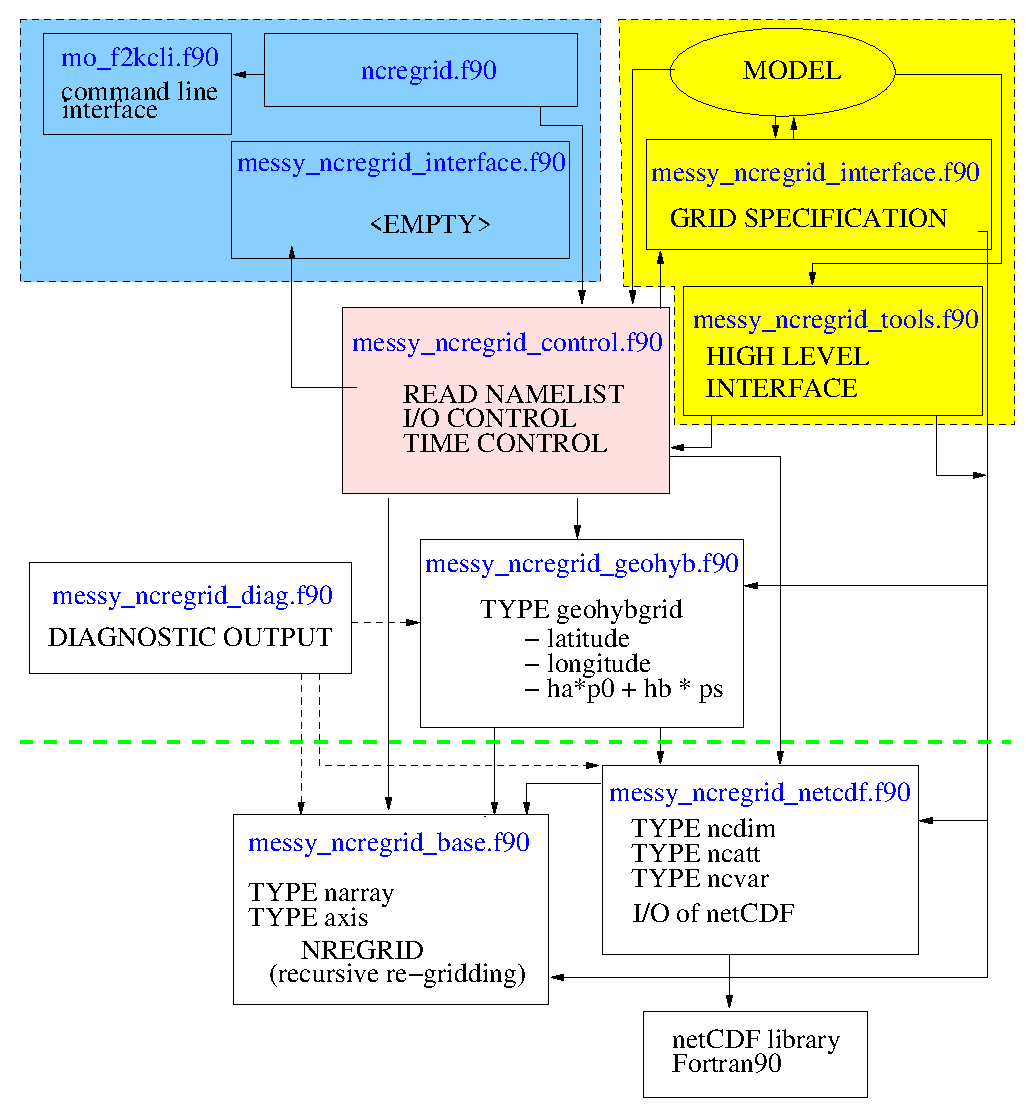
\includegraphics[width=14cm]{overview}}
  \caption[Overview of the different NCREGRID modules]
          {The figure gives an overview of the different NCREGRID modules
           with TYPE declarations and dependencies. The blue shaded parts are
           only needed for the stand-alone mode. The yellow shaded
           areas are required for the coupling to a model.
           Modules below the green dashed line are independent
           on the special requirements of geo-hybrid grids, and can
           be applied to different grid-types.}
  \label{fig:overview}
\end{figure}
%

\subsection{Sequence of operations}
\label{sec:opseq}
%%%%%%%%%%%%%%%%%%%%%%%%%%%%%%%%%%%%%%%%%%%%%%
Figure~\ref{fig:control} shows the steps between reading a namelist
and the resulting output.
%
\begin{figure}
  \centerline{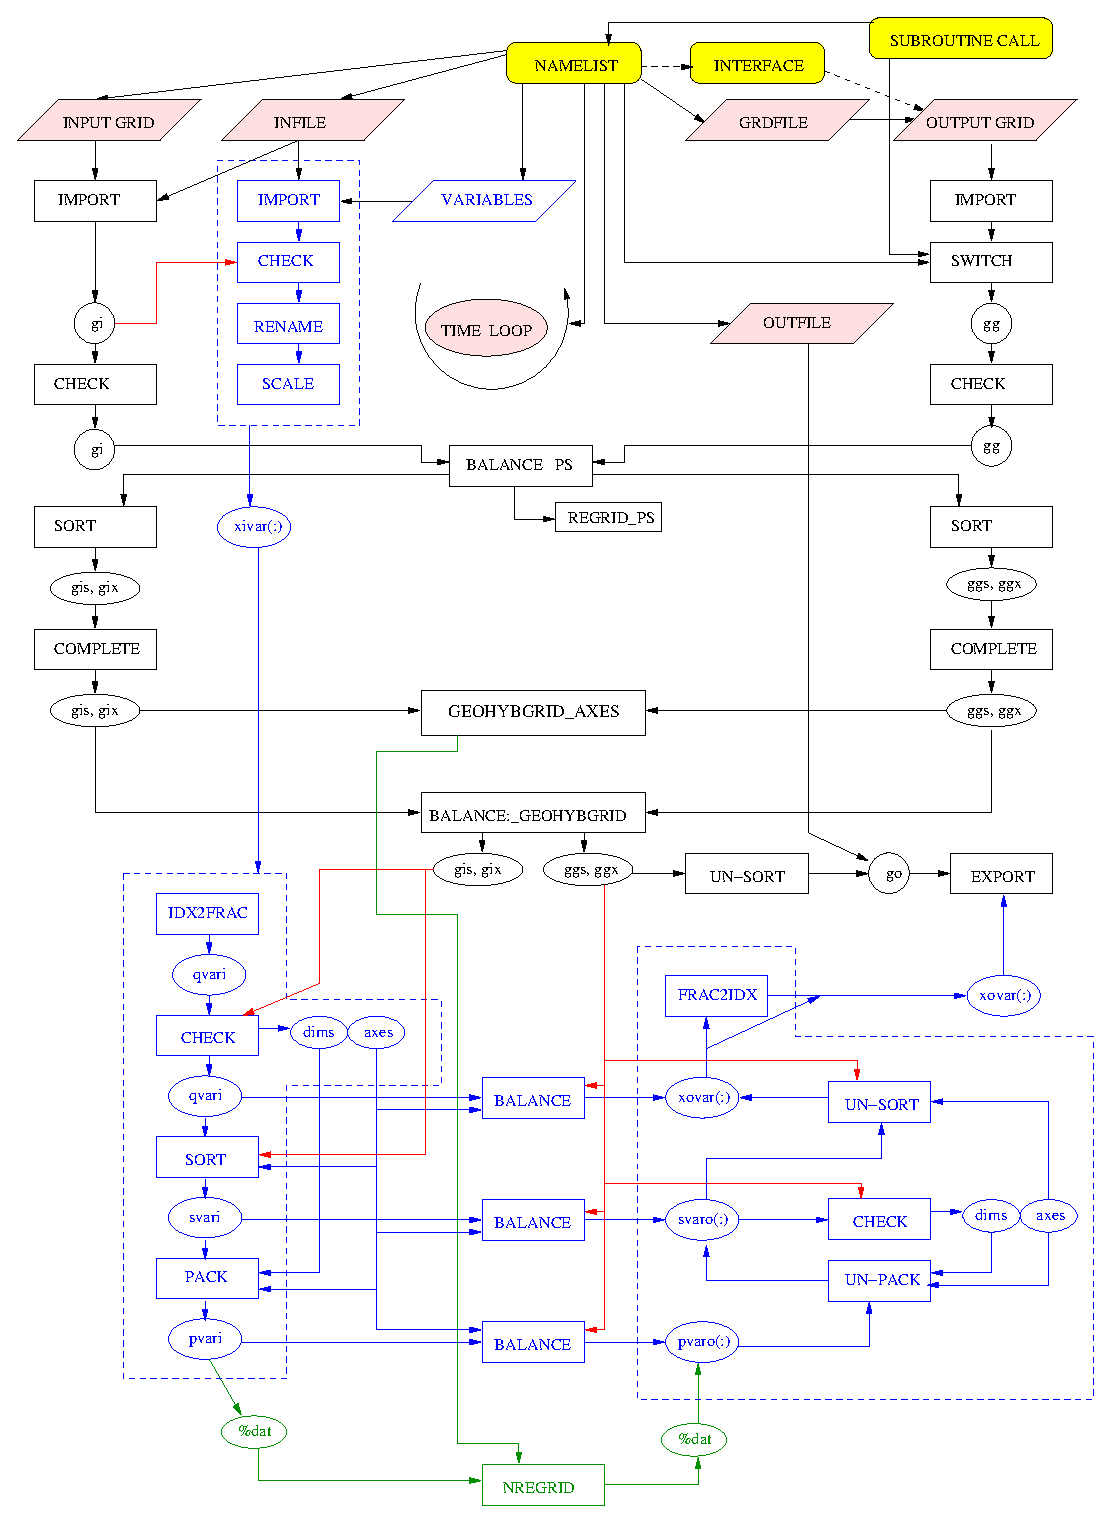
\includegraphics[width=14cm,height=15cm]{control}}
  \caption[NCREGRID Sequence of operations]
          {The figure shows the sequence of operations in NCREGRID. Boxes show
           operations, circles/ellipses show information stored
           in structures (given are the used Fortran95 variable names).
           Dashed boxes surround 
           operations within a loop over variables.
           Black lines are used for operations on grid
           structures, blue lines are used for operations on data variables,
           and red lines indicate connections between grid structures and
           data variables.
           Shown in green is the core regridding step.
           The yellow shaded boxes present the three possibilities
           for user interaction (The grid specification
           via INTERFACE and the options of SUBROUTINE CALL
           are only accessible in the interface mode of NCREGRID).
           Finally, the red boxes show the basic information
           derived from the namelist.
          }
  \label{fig:control}
\end{figure}
%
During the process, input and output grid are 
\begin{itemize}
  \item checked for consistency,
  \item reordered to achieve monotonous axes for NREGRID,
  \item completed (i.e., box-mids are calculated from interfaces, or
        vice-versa).
\end{itemize}

Furthermore, the grid-information of the input ($<$infile$>$)
and output grid ($<$grdfile$>$ or
{\bf INTERFACE\_GEOHYBGRID}) is balanced, such that everything which is
not specified for the output grid is taken from the input grid.
This allows, e.g., a horizontal regridding of 3D (spatial) scalar fields,
while conserving the vertical hybrid-coordinate system of the source file.
In a similar way, only vertical regridding can be performed.

Furthermore, if the surface pressure of the output grid is
not available (or should not be used!), the input surface pressure
is pre-regridded and used for the output grid. Similarly, the
output surface pressure (in $<$grdfile$>$) is used, if the input
surface pressure is omitted. ({\bf BALANCE\_GEOHYBGRID\_PS}).

This balancing allows a flexible handling of the data for many purposes.

\subsection{TYPE definitions}
\label{sec:struct}
%%%%%%%%%%%%%%%%%%%%%%%%%%%%%%%%%%%%%%%%%
Figure~\ref{fig:types} shows in detail the various TYPE definitions
in the different modules and their inter-connections.
%
\begin{figure}
  \centerline{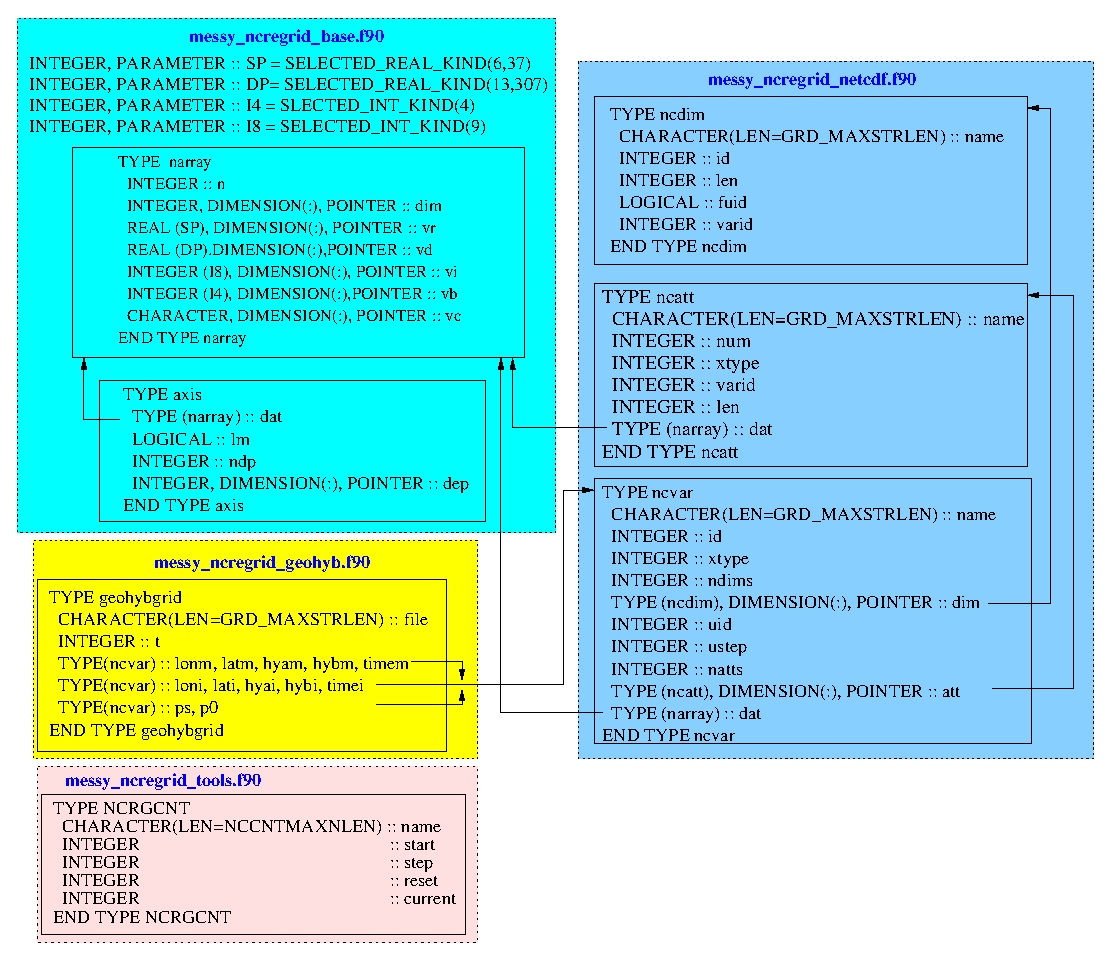
\includegraphics[width=14cm]{types}}
  \caption[NCREGRID type definitions]
          {The figure shows the various type definitions
           (Fortran95 structures) of the different modules
           and their dependencies.
          }
  \label{fig:types}
\end{figure}
%
\begin{itemize}
%
 \item {\bf TYPE narray} ({\it messy\_ncregrid\_base.f90}) provides
       a container for data fields of arbitrary rank $N$
       ($N$-dimensional data) and type
       (float, double precision, integer, byte, character).
       {\bf n} is the rank $N$ of the {\bf narray},
       i.e., the number of dimensions, and
       {\bf dim} an integer vector of length {\bf n} containing the dimension
       length(s). The pointers point to the memory containing the field data,
       organised as a 1-dimensional array.
       %
       The module {\it messy\_ncregrid\_base.f90} provides the 
       \begin{verbatim}
             INTEGER FUNCTION POSITION(dim, vec)
       \end{verbatim}
       which calculates for the element with integer position vector
       {\bf vec(:)} the position {\bf m} in the linear data array,
       if the array is interpreted as an $N$-dimensional array with
       dimension length(s) {\bf dim(:)}.
       The reverse procedure is provided by the
       \begin{verbatim}
             SUBROUTINE ELEMENT(dim, m, vec)
       \end{verbatim}
       This construction is required, since in Fortran95 the rank of an array
       cannot be defined at runtime.
%
 \item {\bf TYPE axis} ({\it messy\_ncregrid\_base.f90}) contains the discrete
       values of an arbitrary axis.
       The logical {\bf lm} is .TRUE. for modulo-axes. Further, 
       {\bf ndp} is the number of dependencies,
       which is 1 for independent axes (such as longitude and latitude),
       and $>0$ for curvilinear axes (such as, e.g., pressure levels, which
       depend for hybrid-grids on latitude, longitude, (and time)).
       The integer vector {\bf dep(:)} contains the numbers (indices)
       of the dependent axes, if the axes are combined in a list of
       \begin{verbatim}
             TYPE (axis), DIMENSION(:), ALLOCATABLE/POINTER
       \end{verbatim}
%
\item {\bf TYPE ncdim}, {\bf TYPE ncvar}, and {\bf TYPE ncatt}
      ({\it messy\_ncregrid\_nc.f90}) provide three Fortran95 structures
      for handling the contents of a {\it netCDF} file
      (see {\it netCDF} manual), namely
      dimensions, variables, and attributes, respectively.
      %
      This module also contains powerful, robust routines for
      {\it netCDF} input/output into/from these structures, such as
      \begin{verbatim}
             SUBROUTINE IMPORT_NCDIM(...)
             SUBROUTINE EXPORT_NCDIM(...)
             SUBROUTINE IMPORT_NCATT(...)
             SUBROUTINE EXPORT_NCATT(...)
             SUBROUTINE IMPORT_NCVAR(...)
             SUBROUTINE EXPORT_NCVAR(...)
      \end{verbatim}
%
\item {\bf TYPE geohybgrid} ({\it messy\_ncregrid\_geohyb.f90}) defines
      the geo-hybrid-grid structure, using {\it netCDF} variables
      ({\bf TYPE ncvar}) for the grid box mid points ({\bf ...m}) and the
      grid box interfaces ({\bf ...i}).
      %
      {\bf t} is the time-step of the current grid, and {\bf file}
      the {\it netCDF} filename for I/O.
%
\item {\bf TYPE ncrgcnt} ({\it messy\_ncregrid\_tools.f90} provides a
      structure for the cyclic event counting, as described in
      section~\ref{sec:level2_2}.
%
\end{itemize}

\subsection{The recursive core of NCREGRID}
\label{sec:nregrid}
%%%%%%%%%%%%%%%%%%%%%%%%%%%%%%%%%%%%%%%%%%%
The actual regridding is performed by the
\begin{verbatim}
    RECURSIVE SUBROUTINE NREGRID(...)
\end{verbatim}
in module {\it messy\_ncregrid\_base.f90}. The algorithm has to be recursive
in order to allow a regridding along an arbitrary number of dimensions.

On the first recursion level, some basic checks on the input are performed.
NREGRID compares the input/output axes and specifies a dimension
as invariant, if the output axis is undefined. Along invariant dimensions,
no regridding is required.
If a dimension is invariant and the respective axis is dependent
(i.e., curvilinear), the axis data is pre-regridded.
The whole regridding procedure requires a special
order of the dimensions, which is calculated by NREGRID itself
(on the first recursion level): first, all independent, non-invariant
dimensions, next all dependent, non-invariant dimensions, and finally all
invariant dimensions.
 
If the current dimension is non-invariant,
NREGRID calculates the overlap - matrices (as fractional overlap)
between source and destination axis. For each non-zero element of
these matrices, it branches to the next recursion level (i.e., to the
next dimension).

If the current dimension is the first invariant dimension, NREGRID
loops along all remaining (invariant) dimensions
and calculates the results for the output grid, depending on the
regridding type (RG\_TYPE) (see section~\ref{sec:rgtypes}).

Since in most practical cases, regridding is performed for more than one
variable on the same grid (axes), NREGRID handles a list of variables in one
step.
The innermost loop is over the number of variables, in oder to increase the
performance, i.e., to avoid recalculation of the same overlap-matrices
for all variables separately.

%%%%%%%%%%%%%%%%%%%%%%%%%%%%%%%%%%%%%%%%%%%%%%%%
\clearpage

\section*{Acknowledgements}
\pdfbookmark[1]{Acknowledgements}{ack} 
\begin{itemize}
\item Rolf Sander (MPI for Chemistry, Mainz)
      for implementation in ECHAM-5, testing the code, and comments on this
      documentation
\item Philip Stier (MPI for Meteorology, Hamburg)
      for implementation in ECHAM-5 and testing the code
\item Huisheng Bian (Dept. of Earth System Science, Univ. of California,
      Irvine)
      for valuable bug-reports of the version 0.8b
\item Benedikt Steil (MPI for Chemistry, Mainz)
      for bug reports
\item Pascal Terray (Laboratoire d'Oc$\acute{\rm e}$anographie
      Dynamique et de Climatologie)
      for reporting the successful installation on SGI
\item Frank Peacock
      for reporting the successful installation on Windows 98
\item Maarten van Aalst
      for reporting the successful installation on SGI, IRIX 6.5
\item Norman Wood (Colorado State University)
      for pointing out the Fortran95 extensions used in the code
\item Ingo Kirchner (FU-Berlin)
      for reporting the successfull installation on PC-Linux with the
      NAG compiler
\end{itemize}

\end{document}
